\section{Experimental protocols}
\label{app:protocols}

\subsection{Trajectory collection and temporal interface}
\label{app:collection}

Each two-tunnel scenario randomizes portal geometry, color--position pairing,
agent start, target leaf, and target position.  Collection generated 55,000
paired hidden/visible scenarios with a 500-step cap and retained the first
50,000 for which both scripted routes succeeded; the active corpus is the
first 10,000 episodes (651,357 stored steps), each ending in success. Scenario
seeds equal 41021 plus the episode index; each condition's policy random-number
generator is initialized once with seed 41021.

The visible-condition collector uses a scripted cue-aware oracle that queries
the scenario pairing, chooses the hub portal paired
with the target leaf, and follows unit-vector waypoints, using a left-lane
waypoint when needed to avoid triggering a non-target portal.
Independent $\mathcal N(0,2^2)$ noise is added to each 2-D action component,
then components are clipped to $[-1,1]$; with probability .05, the previously
executed action replaces the new action.  Before collision and portal handling,
the proposed displacement is the clipped action times 5 pixels.  Shape redraws
the same portals as neutral
triangle/diamond markers, while green/blue replaces orange with blue.
Geometry, actions, targets, rewards, and episode boundaries are unchanged;
image pixels and cue metadata change with the rendering.

Collection stores every primitive step.  Training constructs four-frame
clips with up to three context observations at
\texttt{frameskip}=5 and predicts all three shifted target intervals.
For each latent transition the five intervening 2-D
actions are preserved and flattened to a 10-D action block. MPC therefore
sets \texttt{action\_block}=5: each latent planning step
contains five potentially different primitive actions. Action blocks preserve
these actions rather than repeating a single action; the collector's .05
previous-action repeat probability is a separate perturbation.

Probe fitting and evaluation use disjoint episodes from the same corpus used
for world-model training. The world-model split is defined over clips and
does not exclude probe-test
episodes. These probes consequently measure accessibility in frozen
representations, rather than generalization to episodes unseen during
world-model training. We standardize features on the 640-example union of
fit and validation examples before fitting affine ridge probes with penalty
$\alpha=10$ and evaluating on 256 test examples. We compute $R^2$ separately for each coordinate and average over the same
endpoints as MAE. The standard Color four-endpoint constant MAE is 31.19 px; its two-hub constant is
30.02 px.  Raw patches, selected global states, projected states, and predicted
states are reported separately wherever stagewise claims are made.

\subsection{Rank-based planning protocol}
\label{app:planning}

Evaluation samples portal geometry and pairing, a valid hub start, a target
leaf, and a valid position in that leaf. The goal image renders the agent at
this target in the same layout. Goals are not chosen from recorded trajectories
at \texttt{goal\_offset\_steps=25}; the 25-step planning horizon below is separate.

We rank the two hub entrances by Euclidean distance from the initial agent
position, breaking ties by endpoint index. R1 means the nearer entrance
reaches the goal room; R2 means the farther one does. Ranks describe tasks,
not fixed colors or tunnel identities. Scenarios are sampled before rank
stratification, which retains 25 oracle-solvable cases per rank.

Both planners minimize
$\lVert\hat z_{t+5}-z_{\mathrm{goal}}\rVert_2^2$, summed over projected-state
dimensions.  A planning step contains five consecutive 2-D primitive actions,
so horizon 5 spans 25 primitive steps; receding horizon 5 executes all 25
before replanning unless the episode terminates.  CEM draws 300 Gaussian
sequences per iteration from an
initial zero-mean, unit-variance distribution, forces one sample to the mean,
keeps 30 elites, and refits mean and standard deviation for 30 iterations.  GD
optimizes 100 initial sequences for 30 AdamW steps at learning rate .1; the
first starts at zero and the other 99 receive unit-scale Gaussian noise; added
action noise is zero and gradient clipping is disabled.  Both use seed 3072
and solver sub-batch size one.  Optimized normalized coordinates are not
box-projected; they are inverse-standardized before execution, and the
environment clips each 2-D action to $[-1,1]^2$.

Evaluation uses agent speed 5, batches 10 environments, and allows 400
primitive steps (at most 16 planning calls).  Success is terminal entry within
strict center distance $<16$ px of the requested target; timeouts and
truncations are failures. Fixed, hashed rank manifests specify all evaluation
cases. The scripted
oracle verifies each case in both hidden-search and visible-direct modes
against its expected portal-entry trace.

The primary Color, Shape, and Palette planning evaluations, coordinate probes, and
static landscapes use the same exported epoch-10 spatial $8\times8$ + IDM
3.125 checkpoints. In Figure~\ref{fig:variant-decoders}, Color and Shape snapshots come from
the first batch of the final training epoch, preceding the exported
checkpoint. Palette snapshots come from validation after the final epoch.
We retain frame index 2 of all six clips per run; clip populations and
capture times differ, so this is a qualitative comparison. Color uses BF16 evaluation and filled 18-pixel
markers, matching its training/probe rendering. Shape uses a separate
rank manifest with 20-pixel shape markers. Color and Shape originate from
different source revisions. Palette uses a later implementation with the
same nominal training recipe and filled 18-pixel green/blue markers. Its
evaluation retains the historical CEM/GD solvers and Color case geometry,
changing the cue palette. This aligns solver settings and cases while
leaving source revision as a comparison limitation. Archived configurations
and checkpoint hashes identify the conditions.

For R1 and R2 respectively, Color succeeds on 20/25 and 4/25 cases with
CEM, and 16/25 and 13/25 with GD. Shape succeeds on 22/25 and 6/25 cases
with CEM, and 19/25 and 10/25 with GD. Palette succeeds on 20/25 and
7/25 cases with CEM, and 21/25 and 8/25 with GD. The six matched CLS checkpoints in
Table~\ref{tab:matchedidm} have no corresponding planning evaluation.

\paragraph{Required cues and entrance choices.}
The cue columns of Table~\ref{tab:variantrankplanning} group episodes by the cue
on the entrance that leads to the requested goal room, not by the entrance
actually chosen. Green in Color and Palette, and Triangle in Shape, each
have 12 R1 and four R2 cases; Orange, Blue, and Diamond each have 13 R1 and
21 R2 cases. Thus the pooled cue rates compare different mixtures of ranks.
These descriptive strata were formed after evaluation and do not establish
a preference for a particular color or shape. Each variant uses one model
checkpoint, and the four-case R2 strata are especially imprecise.
Table~\ref{tab:cuebyrank} gives the full breakdown: success is lower on R2
for every cue and both planners.

\begin{table}[!htbp]
\centering
\caption{\textbf{Success falls on the farther entrance for both cue identities.}
Task success (\%) by the cue required to reach the goal room.
$n_1/n_2$ gives R1/R2 case counts; All pools both ranks.
Cue groups have unequal rank support, including only four R2 cases for
Green/Triangle.}
\label{tab:cuebyrank}
\renewcommand{\arraystretch}{1.08}
\setlength{\tabcolsep}{3pt}
\begin{tabular*}{\linewidth}{@{\extracolsep{\fill}}llrrrrrrr@{}}
\toprule
Variant & Required cue & $n_1/n_2$ & \multicolumn{3}{c}{CEM success $\uparrow$} & \multicolumn{3}{c}{GD success $\uparrow$} \\
\cmidrule(lr){4-6}\cmidrule(l){7-9}
 & & & All & R1 & R2 & All & R1 & R2 \\
\midrule
Color & Green & 12/4 & 56.3 & 75.0 & 0.0 & 62.5 & 66.7 & 50.0 \\
 & Orange & 13/21 & 44.1 & 84.6 & 19.0 & 55.9 & 61.5 & 52.4 \\
\addlinespace[2pt]
Shape & Triangle & 12/4 & 68.8 & 91.7 & 0.0 & 56.3 & 66.7 & 25.0 \\
 & Diamond & 13/21 & 50.0 & 84.6 & 28.6 & 58.8 & 84.6 & 42.9 \\
\addlinespace[2pt]
Palette & Green & 12/4 & 56.3 & 75.0 & 0.0 & 75.0 & 91.7 & 25.0 \\
 & Blue & 13/21 & 52.9 & 84.6 & 33.3 & 50.0 & 76.9 & 33.3 \\
\bottomrule
\end{tabular*}
\end{table}

To test whether proximity influences entrance choice, we also inspect the
first actual hub-to-leaf teleport in each episode. On R2, the nearer entrance
is incorrect by construction. Table~\ref{tab:firstentrance} shows that CEM
usually enters it first, whereas GD is more mixed: on Color, GD chooses
the nearer entrance in 13 cases and the farther one in 12. Episodes with
no hub entry remain in the denominator. First entrance and final success
measure different behaviors: an agent can recover after entering the wrong
room, or enter the correct room but fail to reach the goal position.
A 50\% success rate therefore does not establish chance-level tunnel
choice; no random-policy task-success baseline is measured here.

\begin{table}[!htbp]
\centering
\caption{\textbf{The nearer, wrong entrance is often chosen first on R2.}
Counts out of 25 episodes per row. Columns are mutually exclusive and
include every episode. These are actual teleport events, not visits near
a portal.}
\label{tab:firstentrance}
\begin{tabular*}{\linewidth}{@{\extracolsep{\fill}}llrrr@{}}
\toprule
Variant & Planner & Nearer (wrong) & Farther (correct) & No entry \\
\midrule
Color & CEM & 22 & 1 & 2 \\
 & GD & 13 & 12 & 0 \\
Shape & CEM & 19 & 5 & 1 \\
 & GD & 14 & 9 & 2 \\
Palette & CEM & 18 & 7 & 0 \\
 & GD & 18 & 7 & 0 \\
\bottomrule
\end{tabular*}
\end{table}

\section{Energy-map construction}
\label{app:landscapes}

We fix one layout and place the agent at the 210 valid centers of a
$20\times20$ image grid, holding tunnel positions and cues unchanged.
For each goal image, the learned energy $E$ is the squared distance between
the frozen projected features of the current observation and the goal.
The geodesic reference energy is the shortest remaining walking distance
through the true paired tunnels, computed on a navigation graph that follows
the environment's portal-entry and re-entry rules; teleportation adds no
walking distance. We evaluate both maps at the same positions and interpolate
within each room for display. Yellow indicates low energy, with a shared
scale across the two goals in each column. Learned energy uses squared
feature units; the reference uses pixels. These maps compare observed states;
the planner applies the learned energy to predicted states. The implementation
and saved map values accompany the code.

\FloatBarrier
\section{Transition-diversity ablation}
\label{app:exposure}

\paragraph{Hypothesis and exposure counts.}
A visible cue does not necessarily contribute equally to every prediction
error. In Tunnel Room, most trajectory steps approach a portal, whereas
its cue-dependent destination is observed at a crossing. The 10,000-episode
corpus contains 641,357 raw transitions, of which 12,180 (1.90\%) are
crossings. Its 463,033 legal training clips produce 1,389,099 target intervals.
After accounting for overlapping clips and frameskip, crossing-adjacent
exposure is 8.95\%, while approach motion occurs in 81.6\% of target intervals.
An interval can contain both events. This imbalance motivates the hypothesis
that average prediction favors spatial regularities over cue-dependent
outcomes; it does not establish the cause of the observed readout gap.

\paragraph{Intervention and results.}
An earlier Color pilot, using a spatial readout and IDM weight 3.125, adds
transition-centered windows equal to 10\%, 50\%, or 100\% of the original
training set. Selected decoder outputs appear more saturated and show
stronger color separation (Figure~\ref{fig:diversity}). Coordinate probes do
not show a corresponding consistent improvement: current-state cue $R^2$
is .224, .222, .174, and .200 at 0/10/50/100\% additional windows; predicted-state
scores are .226, .244, .213, and .231. Four-endpoint cue MAE remains in the
27.2--28.1 px range. Keeping epochs fixed also increases compute by
approximately $1.1\times$, $1.5\times$, and $2\times$.

\paragraph{Interpretation and follow-up.}
More saturated reconstructions do not establish cue binding: distinct colors
can still be assigned to the wrong endpoints. Frames differ across conditions,
and increased optimization may contribute to their appearance. A controlled
follow-up should fix the training budget and evaluate identical held-out
examples for saturation, identity, cue-conditioned localization, and planning.
Cue swaps and portal-crossing rollouts can then test whether visual recovery
changes predicted destinations or actions.

\begin{figure}[ht]
  \centering
  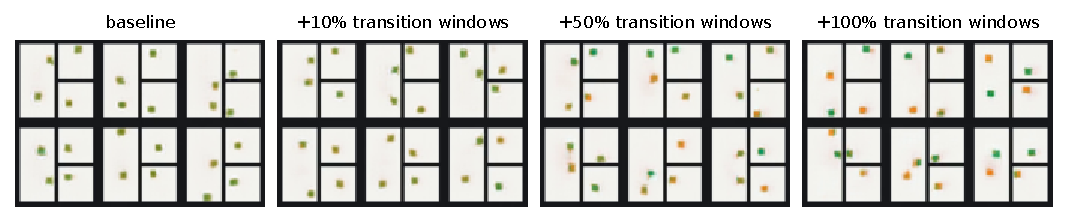
\includegraphics[width=\linewidth]{figures/lewm_transition_diversity_decoder.pdf}
  \caption{\textbf{Transition-focused sampling changes decoder appearance.}
  Selected reconstructions appear more saturated, but frames differ across
  conditions and cue identity is not measured. Coordinate $R^2$ does not
  improve consistently; added windows increase compute.}
  \label{fig:diversity}
\end{figure}

\FloatBarrier
\section{Additional readout diagnostics}
\label{app:diagnostics}

\begin{figure}[h]
  \centering
  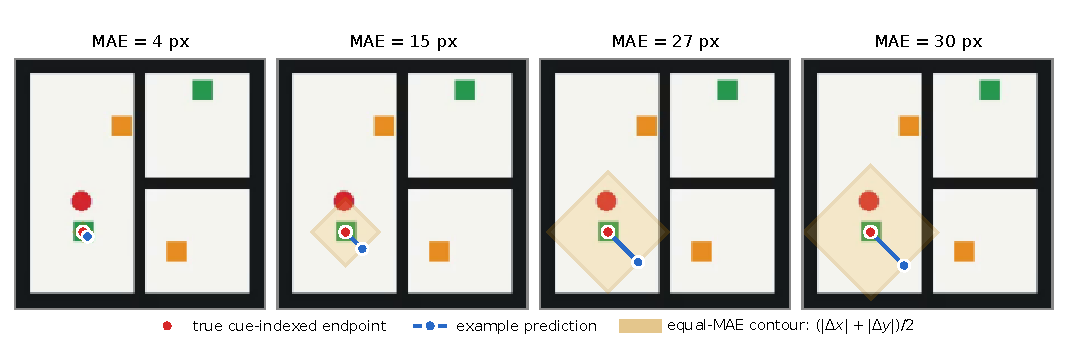
\includegraphics[width=.80\linewidth]{figures/tr2_color_mae_scale.pdf}
  \caption{\textbf{Coordinate error at the task scale.} The gold contour
  marks predictions with a fixed per-coordinate MAE; the blue point is one
  illustrative prediction. From left to right, the panels show 4 px
  (approximately the spatial Color location error), 15 px (a coarse-error
  example), 27 px (approximately the cue-coordinate error), and 30 px
  (an illustrative constant-baseline error). The task-specific constant baseline and
  $R^2$, not a universal pixel threshold, determine the interpretation.}
  \label{fig:mae}
\end{figure}

\paragraph{Visible hue remains accessible in patch tokens.}
A separate binary hue-classification audit of a historical Color+IDM checkpoint
achieves 100\% balanced accuracy from native patch tokens but 45.3\% from the
projected state (chance 50\%), using an episode-disjoint validation split.
This contrast localizes an accessibility gap along the compact-state
processing path; it does not establish an inability to perceive color.
Differences in feature dimensionality and readout capacity also preclude a
direct claim of information loss.

The hue classifier asks which hue occupies a portal slot; the coordinate
probe asks where a cue-indexed endpoint lies. The hue audit fits on 525
episodes, selects the ridge penalty using 75 validation episodes, and tests
on 150 episodes. The 640/256 coordinate protocol instead fixes the penalty.
Both readouts can miss information outside their chosen function class.
Likewise, MSE decoding can average uncertain outputs: its population optimum
is $d^*(z)=\mathbb E[X\mid z]$, but the representation, decoder capacity, and
optimization can limit the trained decoder.
